% ----------------------------------------------------------------
% AMS-LaTeX Paper ************************************************
% **** -----------------------------------------------------------
\documentclass[9pt]{amsart}
\usepackage{graphicx}
% ----------------------------------------------------------------
\vfuzz2pt % Don't report over-full v-boxes if over-edge is small
\hfuzz2pt % Don't report over-full h-boxes if over-edge is small
% THEOREMS -------------------------------------------------------
\newtheorem{thm}{Theorem}[section]
\newtheorem{cor}[thm]{Corollary}
\newtheorem{lem}[thm]{Lemma}
\newtheorem{prop}[thm]{Proposition}
\theoremstyle{definition}
\newtheorem{defn}[thm]{Definition}
\theoremstyle{remark}
\newtheorem{rem}[thm]{Remark}
\numberwithin{equation}{section}
% MATH -----------------------------------------------------------
\newcommand{\norm}[1]{\left\Vert#1\right\Vert}
\newcommand{\abs}[1]{\left\vert#1\right\vert}
\newcommand{\set}[1]{\left\{#1\right\}}
\newcommand{\Real}{\mathbb R}
\newcommand{\eps}{\varepsilon}
\newcommand{\To}{\longrightarrow}
\newcommand{\BX}{\mathbf{B}(X)}
\newcommand{\A}{\mathcal{A}}
\newcommand{\q}{\mathbf{q}}
\newcommand{\x}{\mathbf{x}}
% ----------------------------------------------------------------





\begin{document}

\title[YARP]{
YARP: Yet Another Ridiculous Paper}%
\author{IIT Robotics Lab}  %


%\keywords{manipulation, grasping, humanoid robotics, motion primitives}%

%\date{}%
%\dedicatory{}%
%\commby{}%
% ----------------------------------------------------------------
\maketitle
% ----------------------------------------------------------------
%\vspace{-0.9cm}
%\begin{center}
%{Robotics Behavioural \& Cognitive Sciences Lab\\ IIT, Italian Institute of Technology, ITALY}
%\end{center}
%\vspace{0.5cm}


\vspace{-0.2cm}
\begin{center}
{\emph{\textbf{Abstract}}}
\end{center}
\vspace{0.2cm}

\emph{In this paper we describe the actuation and control of a humanoid robot neck. Particular attention will be posed on the description of the neck actuation structure, whose design has resulted in a noticeable human similarity. Specifically, the final mechanical design was inspired by the human skeleton, with the neck bone movements constrained and actuated by the surrounding muscles. In our robotic platform, the neck bone was realized with a steel spring surrounded by steel tendons in place of muscles. The specific and innovative mechanical design have imposed the design of a non-standard actuation structure which, in turn, have lead to an innovative control scheme. The main focus of the paper will be on describing different control schemes and discussing their performances in details.} 


\section{Introduction}

Humans exhibit a wide and complex repertoire of movements far beyond the motor capabilities of modern robots. Clearly, the
realization of an artificial system capable of more realistic movements passes trough a series of technological improvements,
especially if we are interested in replicating both kinematic and dynamical aspects. Recently, there has been a growing interest in developing robots whose geometric and actuation structures resemble those of a human being. Probably, one of the most extreme steps in this direction is represented by the robot recently developed by O. Holland and colleagues \cite{Cronos}; another interesting example is the humanoid robot Kotaro \cite{Kotaro}.


\section{Humanoid platform} \label{Sec:Platform}

The robotic platform on which the discussed controller has been implemented is the humanoid robot James \cite{James06}.\\James is a 22-DOF torso with moving eyes and neck, an arm and a highly anthropomorphic hand (see Figure \ref{Fig:PicureJames}). In the following subsections we briefly cover the robot design, its actuation, and sensorization. More details about the neck structure are given in section 3.

\begin{figure}[h!tbp]
\centering
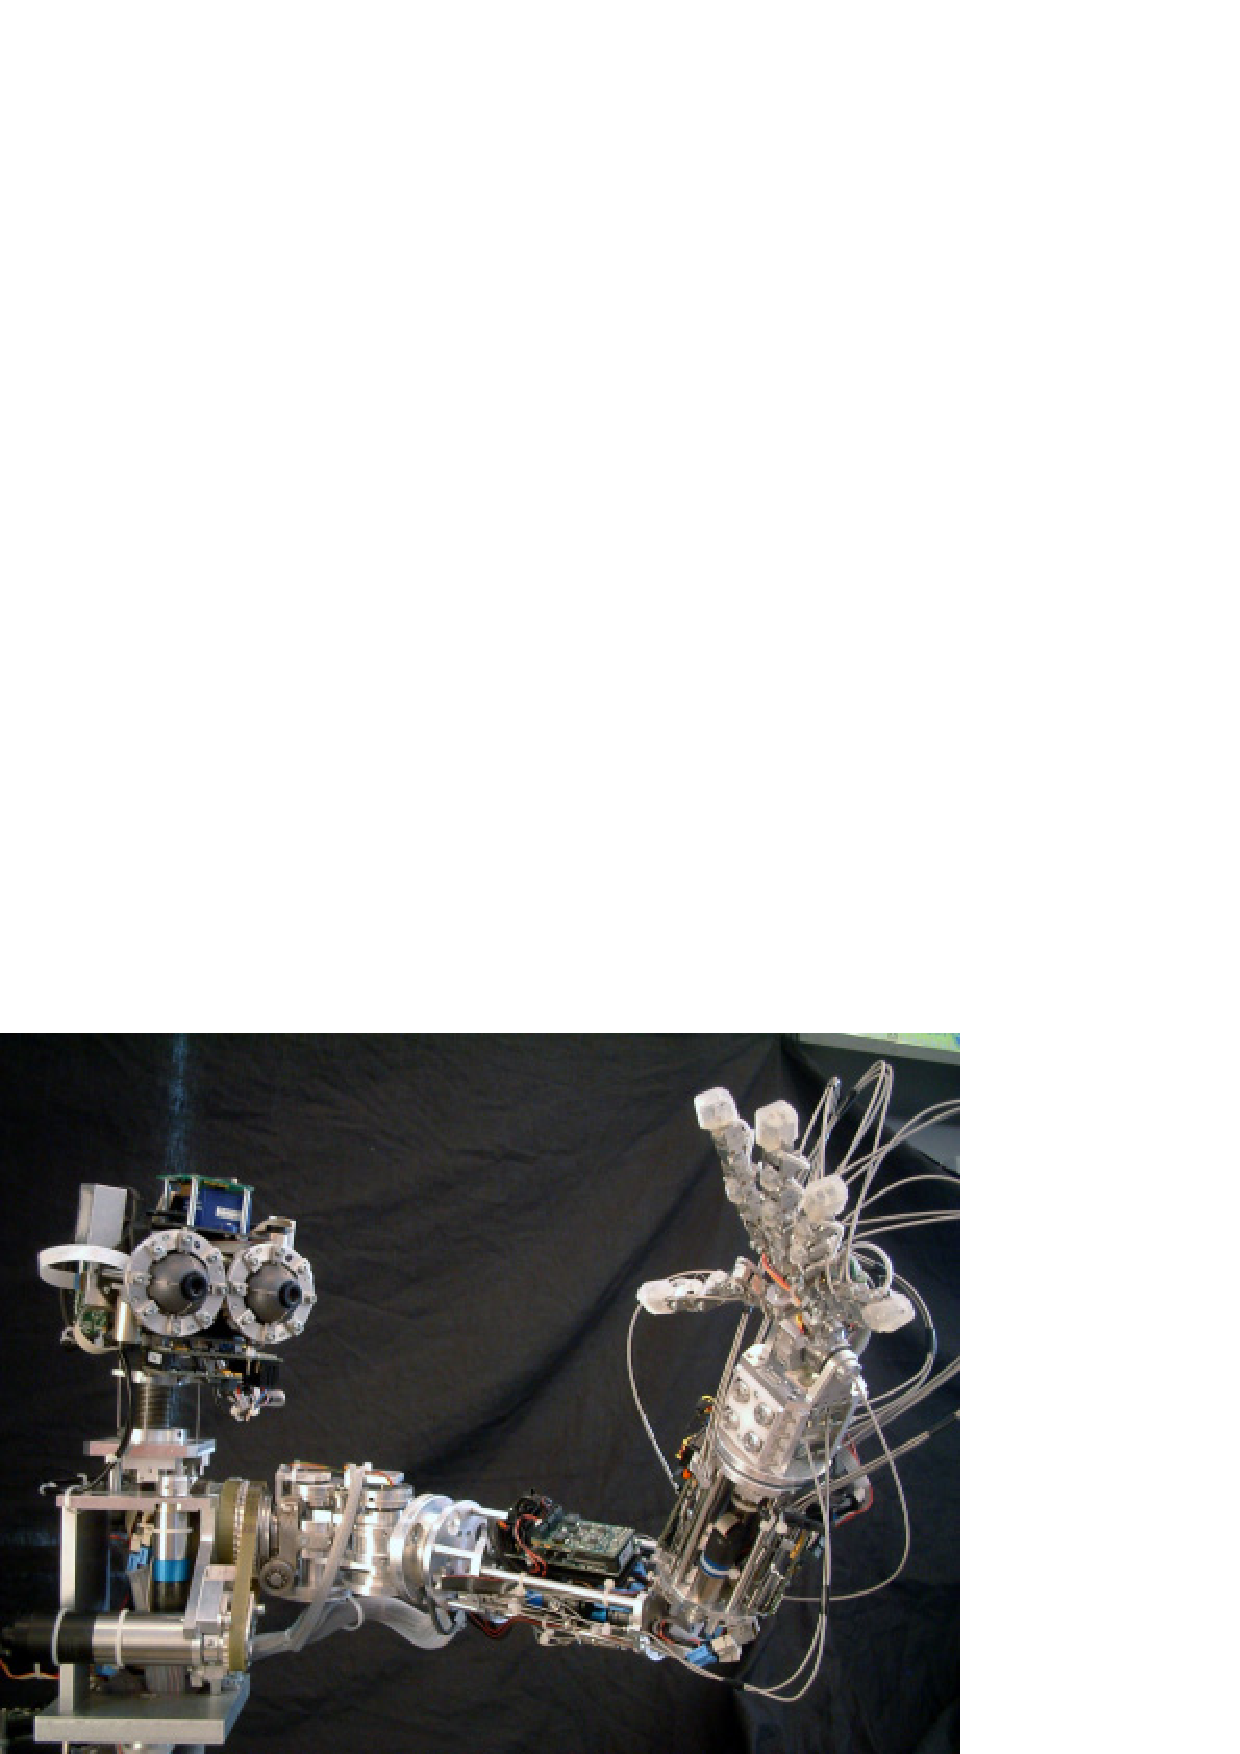
\includegraphics[width=50mm]{image/James1.png}
\caption{The humanoid robot James.}
\label{Fig:PicureJames}
\end{figure}

\subsection{Robot design}

The robot structure is similar to that of humans, both in size (approximatively that of a ten-year-old boy), number of DOFs and range of movements; the total weight (about 8 kg: 2 kg the head, 4 kg the torso and 2 kg arm and hand together) has been kept low by the use of light material such as aluminum and ergal.\\The head is equipped with two eyes, which can pan and tilt independently (4 DOFs), and is mounted on the 3-DOF neck, which allows the movement of the head as needed in the 3D rotational space.\\The arm has 7 DOFs: three of them are located in the shoulder, one in the elbow and three in the wrist. The hand has five fingers, with overall 17 joints coupled among them and actuated by just 8 motors.


\subsection{Actuation system}

The 22 DOFs are actuated by a total of 23 motors, whose torque is transmitted to the joints by plastic toothed belts and stainless-steel tendons, provided with springs at critical locations.\\This solution is appealing for at least two reasons. First, it allows the housing of the motors far from the joints, thus distributing the weights in accordance with the designer wish. Second, the intrinsic elasticity of belts, tendons and springs gives a noteworthy compliance to the whole structure allowing the robot to move safely in a dynamic and unknown environment.

\subsection{Sensory system}

The robot is equipped with vision, proprioception, kinesthetic and tactile inputs. Vision is provided by two digital CCD cameras (PointGrey Dragonfly remote head), located in the eyeballs. The proprioceptive and kinesthetic senses are achieved through position sensors (magnetic incremental encoders connected to all motors); furthermore, a 3-axis orientation tracker (Intersense iCube2) has been mounted on top of the head, to emulate the vestibular system. Tactile information is extracted from several magnetic silicone-made pressure sensors which have been specifically designed and developed for James, placed in the fingers.

\section{Neck structure} \label{Sec:NeckStructure}

The neck is constituted by a steel spring, which holds the head giving it the possibility of bending forward (pitch) and laterally (roll). The actuation of these two degrees of freedom is obtained with a peculiar structure, recalling the design of a parallel manipulator. Specifically, the neck is surrounded by three steel tendons, whose length determine the position of the spring and therefore, the pitch and roll position of the neck. The length of the tendons is adjusted by means of three motors, positioned at the base of the neck (see Figure \ref{Fig:HeadAct}). On top of the spring, a fourth independent motor is mounted, directly actuating a third degree of freedom, the head yaw (i.e. rotation around an axis parallel to the pan axes of the two eyes). In the current paper we are mainly interested in the control of the head pitch and roll by coordinating the movements of surrounding tendons.

\begin{figure}[tbp]
\centering
\includegraphics[width=50mm]{image/HeadAct.pdf} 
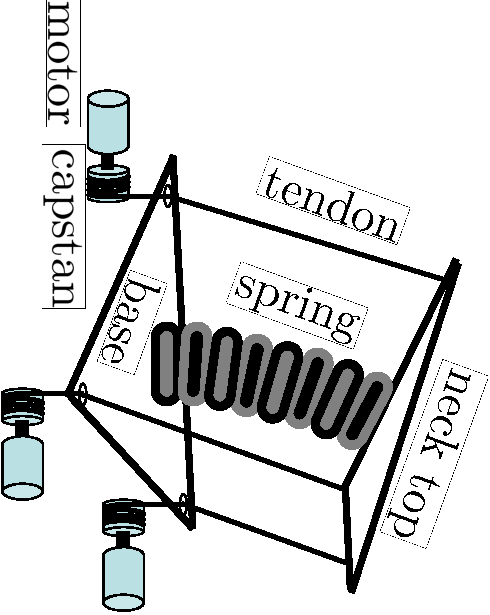
\includegraphics[width=40mm, angle=90]{image/NeckModelScheme.pdf} 
\caption{Neck actuation system and sketch of the neck kinematics. Each motor pulls a tendon which passes trough a hole in the neck base. In this way the effective tendon length can be reduced to bend the spring in different directions.}
\label{Fig:HeadAct}
\end{figure}

\begin{figure}[tbp]
\centering
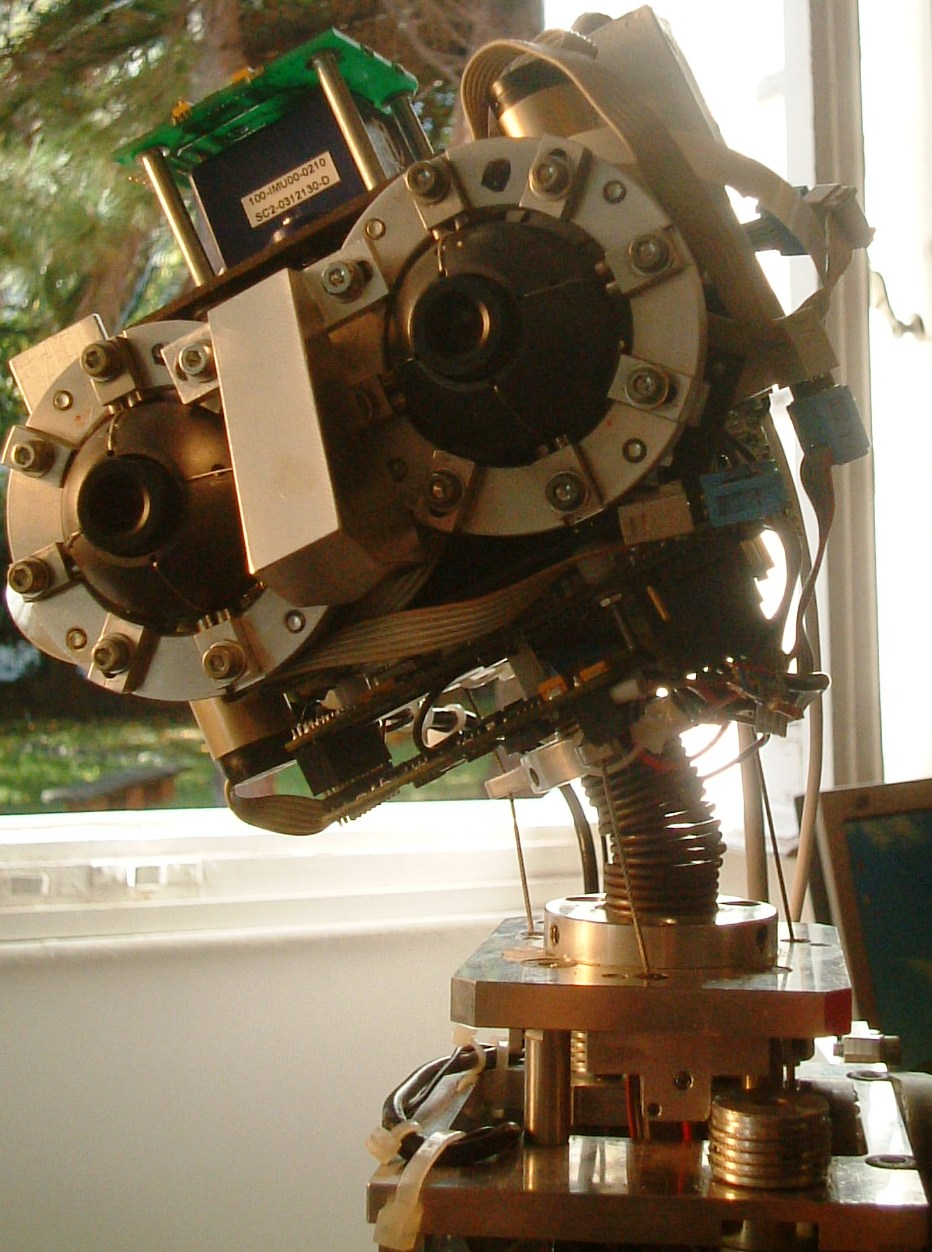
\includegraphics[width=20mm]{image/HeadRight.jpg} \hspace{1pt}
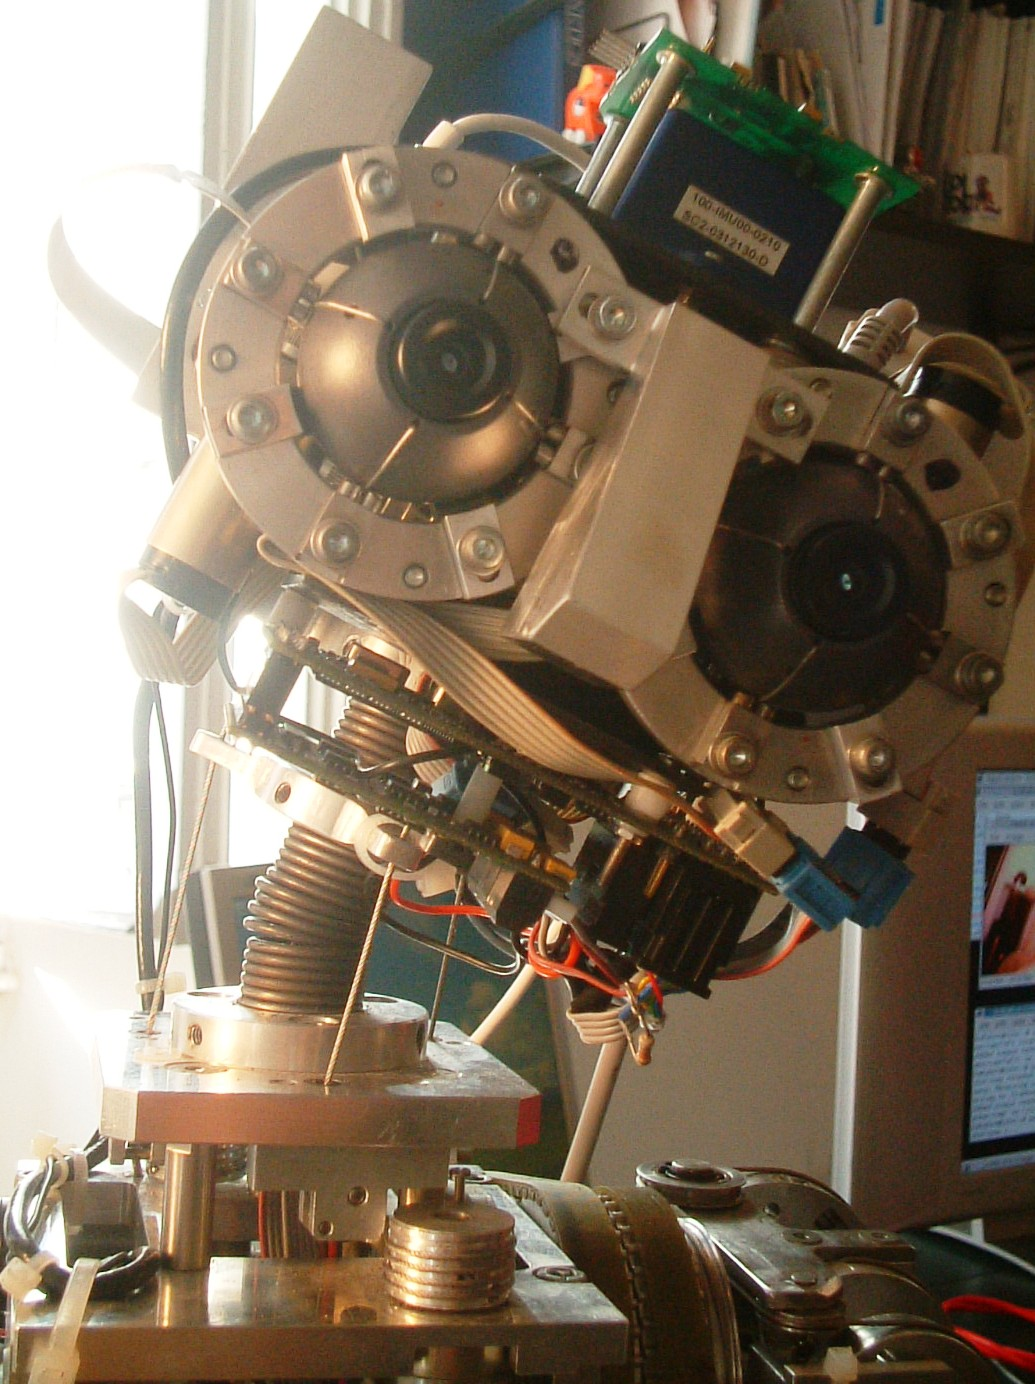
\includegraphics[width=20mm]{image/HeadLeft.jpg} \hspace{1pt}
\includegraphics[width=21mm]{image/HeadAhead.jpg} \hspace{1pt}
\includegraphics[width=20mm]{image/HeadBack.jpg} \hspace{1pt}\\

\caption{James head. Different configurations seen from different views.}
\label{Fig:HeadPos}
\end{figure}


\subsection{Redundancy of the actuation scheme}

Clearly, the above actuation structure is somehow redundant. Practically, the pitch and roll movements (two degrees of freedom) are actuated by three motors. In a mathematical sense, redundancy corresponds to the fact that the same configuration of the system can be achieved by different positions of the actuators. Classical techniques can be used to exploit the advantages of redundant systems \cite{SamsonEspiau}. However, in our case there are additional constraints that will guide the controller design in handling redundancy. 

To understand the structure of the problem, let us reduce the structure to a two dimensional space. In this situation, we have two independent motors to actuate a single degree of freedom, nominally the slope of the surface on which the head is mounted.
Consider first the system whose actuation scheme is given in Figure \ref{Fig:HeadAct2D}. Considering the surface slope as the task of our control, this system is redundant. Roughly speaking, shortening both cables of the same length does not produce any slope movement but only a variation of the spring compression. Classically, this is what we define redundancy in the actuation.
As previously said, in our case there are additional constraints that rule out this redundancy. Practically speaking, the spring at the base of the neck is entirely compressed by the weight of the carried electronics and mechanics\footnote{The description of the system in Figure \ref{Fig:HeadAct2D} is merely for understanding the issue of redundancy. Practically speaking it would be very difficult to model the forward kinematics of this system. The actual system, i.e. the one schematically represented in Figure \ref{Fig:HeadAct2DSpring}, will be much easier to model kinematically. This is the reason why we did not choose a stiffer spring capable of sustaining the head weight.} (motors, cameras, chassis, etc. etc.), as indicated in Figure \ref{Fig:HeadAct2DSpring}. As a consequence of this fact, shortening/lengthening both cables simultaneously no longer produces a variation of the spring compression but only a varies the cable tensions. Remarkably, these tensions should be kept under control: high tensions damage the spring spirals and low tensions cause wrong alignment of the cables on the capstans. Ideally, the tension of the cables can be controlled if we could use some sort of tension sensors. In our system these sensors are not currently available. Therefore, in the present paper we show how to keep the cable tensions under control by means of a kinematic model of the system.

\begin{figure}[tbp]
\centering
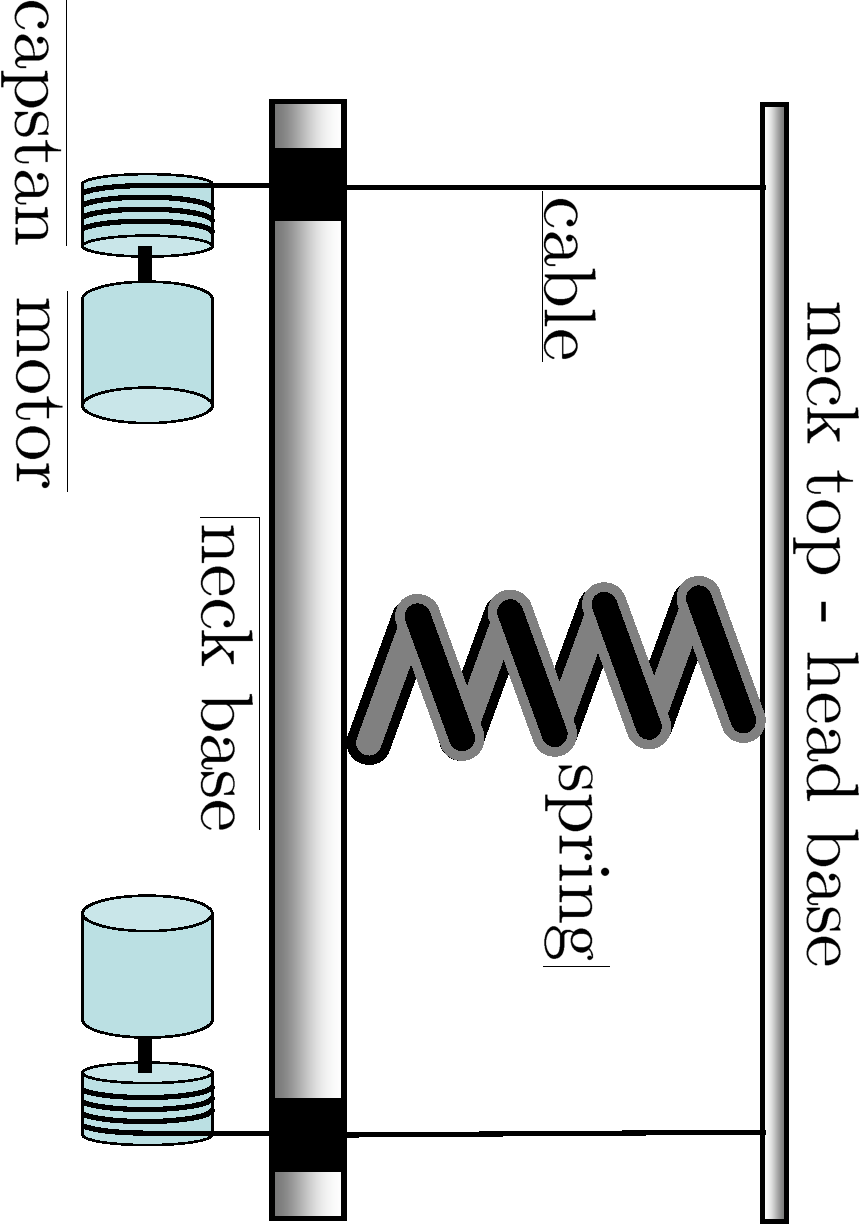
\includegraphics[width=50mm, angle=90]{image/Neck2DSpring.pdf} 
\caption{Two dimensional scheme of an actuation system similar to james's neck.}
\label{Fig:HeadAct2D}
\end{figure}

\begin{figure}[tbp]
\centering
\includegraphics[width=30mm, angle=90]{image/Neck2DSpringCompressed.pdf} 
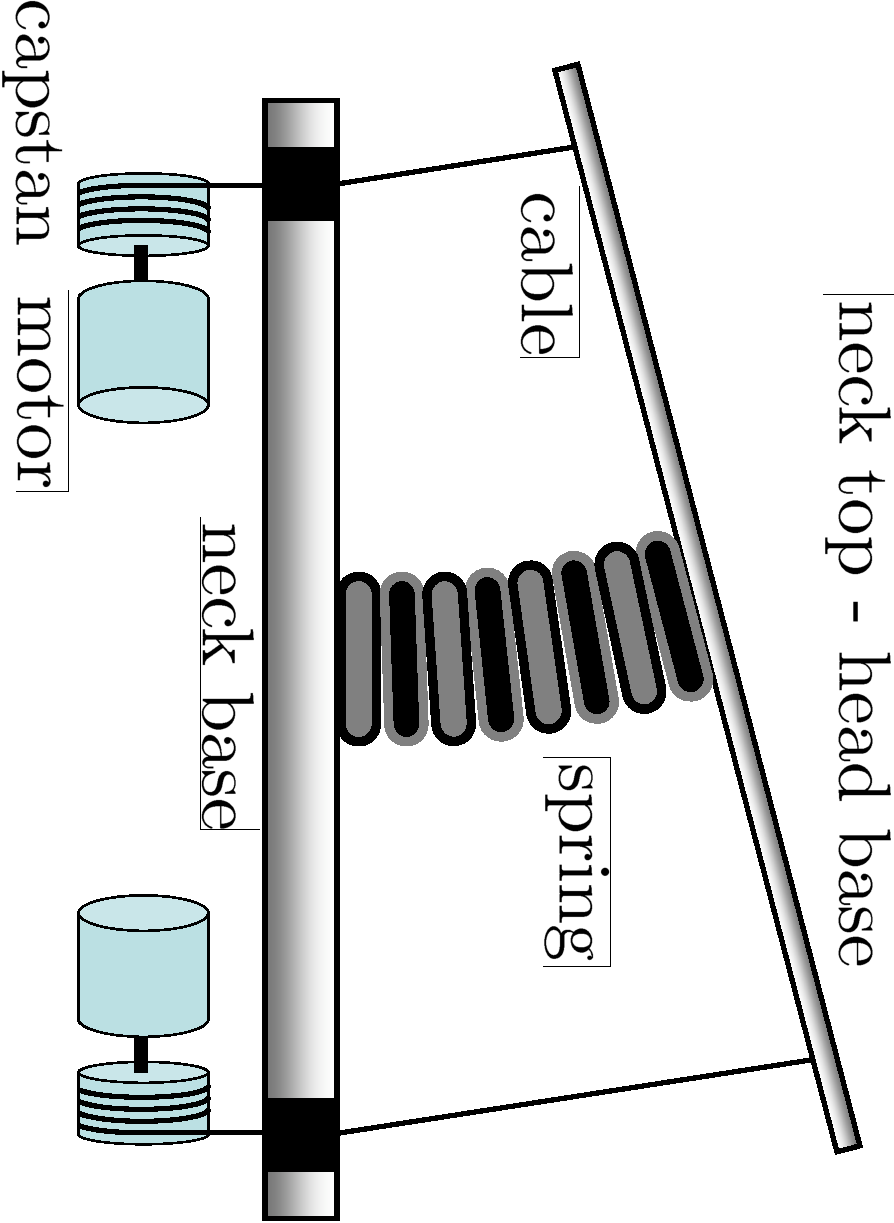
\includegraphics[width=30mm, angle=90]{image/Neck2DSpringCompressedBent.pdf} 
\caption{Equivalent two dimensional scheme of james's neck.}
\label{Fig:HeadAct2DSpring}
\end{figure}


\section{Control of the neck} \label{Sec:NeckControl}

The peculiar structure of the neck has required the design of an original control technique. The final design makes use of the 3-axis orientation tracker positioned on top of the robot neck. Though the given sensor is capable of measuring its absolute rotation along three orthogonal axes, in the given application we used only part of the available information. In particular, we used the measurements corresponding to the head pitch and roll rotations, denoted $\theta_p$ and $\theta_r$ respectively; these rotations corresponds to the degrees of freedom actuated by the three motors at the base of the neck. The third sensor measurement, the yaw rotation $\theta_y$ (a rotation around an axis orthogonal to the ``neck top'' as indicated in Figure \ref{Fig:HeadAct}), will not be used for two reasons: first, it is not influenced by the first three motor positions; second, it can be better measured using the encoder mounted directly on the shaft of the fourth motor.

\subsection{Neck control in details} \label{Sec:NeckControlInDetails}

As already pointed out, the neck structure is characterized by three degrees of freedom: pitch $\theta_p$, roll $\theta_r$ and yaw $\theta_y$. The yaw movement, is directly actuated by a single dc motor; its control is based on a standard PID controller. The control strategy for the remaining two movements will be instead described in details in this section.

The design of the pitch and roll control loops has required the development of a neck structure model \footnote{The model is based on the assumption that the spring has a constant length. Practically, when the spring bends on a side, it maintains its length on that side (remember that the spring is compressed by the head weight) while stretching on the opposite side. When the spring is bent, the assumption is that its curvature is constant along the entire spring length.}.
As already pointed out the system is somehow redundant (3 actuators versus 2 degrees of freedom) but the redundancy needs to be ruled out in order to keep the tendons tension within certain limits and the spring spirals aligned. Practically, because of redundancy, the same neck orientation $\x = [\theta_p$, $\theta_r] \in \mathbb R^2$ (i.e. the orientation tracker measurements) can be achieved with different tendons (cables) configurations $\q = [d_1$, $d_2$, $d_3] \in \mathbb R^3$ (i.e. the position of the motors). Mathematically speaking, the neck forward kinematic are described by a function:
\begin{eqnarray} \label{Eq:Fwd_model_neck}
\x = f (\q) \qquad f:\mathbb{R}^3 \rightarrow \mathbb{R}^2.
\end{eqnarray}
The function $f$ cannot be directly inverted because the same $\x$ can be achieved by different configurations $\q$. Among all these configurations, there is an ideal one $\q^*$ which corresponds to straight tendons and constant curvature of the spring. This configuration can be easily computed (see appendix for details) thus leading to the following:
\begin{eqnarray} \label{Eq:Model_neck}
\q^* = f_{inv} (\x).
\end{eqnarray}
The other tendons configuration corresponding to the same $\x$ are less desirable because of the reasons explained before. The reader should notice that (\ref{Eq:Model_neck}) is a sort of inverse kinematic model\footnote{In absence of modeling errors we have $f(f_{inv}(\x)) = \x$, $\forall \x \in \mathbb R^2$. Notice that the forward counterpart (\ref{Eq:Fwd_model_neck}) is  complicated to be analytically computed and its computation falls outside the scope of this paper.} expressing the configuration of the motors to achieve a desired neck orientation. Geometrically speaking, (\ref{Eq:Model_neck}) defines a two dimensional manifold $\mathcal M$ embedded in the three dimensional space of the cables configurations.
In the remaining of the current section we describe how to control the three motors in order to position the neck on a desired configuration $\x_d$ while keeping the position of the motors as close as possible to the manifold described by (\ref{Eq:Model_neck}).

\subsubsection{Purely model based solution} \label{Sec:ModelBasedSolution}

If the model were perfectly corresponding to the real system, the problem of orienting the neck in a desired configuration $\x_d$ would be easily solved by computing the desired tendons length $\q_d = f_{inv} (\x_d)$ and controlling the positions of the three motors\footnote{The three motors are equipped with encoders so that the motor position control has been easily achieved with a simple PID controller based on feedback from encoders.} so as to regulate the tendons to the desired configuration. Practically speaking, every model has its own errors and therefore the proposed scheme will never orient precisely the neck. In order to check the quality of the model we evaluated the error in positioning the neck in the configuration $\x_d$. Specifically, we computed $\mathbf e = \x - \x_d$ where $\x$ is the sensor measurement after having positioned the motors in the configuration $\q^*_d = f_{inv}(\x_d)$ with the following control law:
\begin{equation} \label{Eq:PurelyModelBasedControl}
\dot{\q} = - K_p (\q - \q^*_d),
\end{equation}
where $K_p \in \mathbb R^{3 \times 3}$ is an arbitrarily chosen gain matrix. Theoretically\footnote{According to what we have seen in the previous section the $f_{inv}$ have the following property $\x = f(f_{inv} (\x_d)) = \x_d$.}, in absence of modeling errors we should have $\mathbf e = 0$; practically, we obtained the errors in Figure \ref{Fig:ErrorModel}.

\begin{figure}[tbp]
\centering 
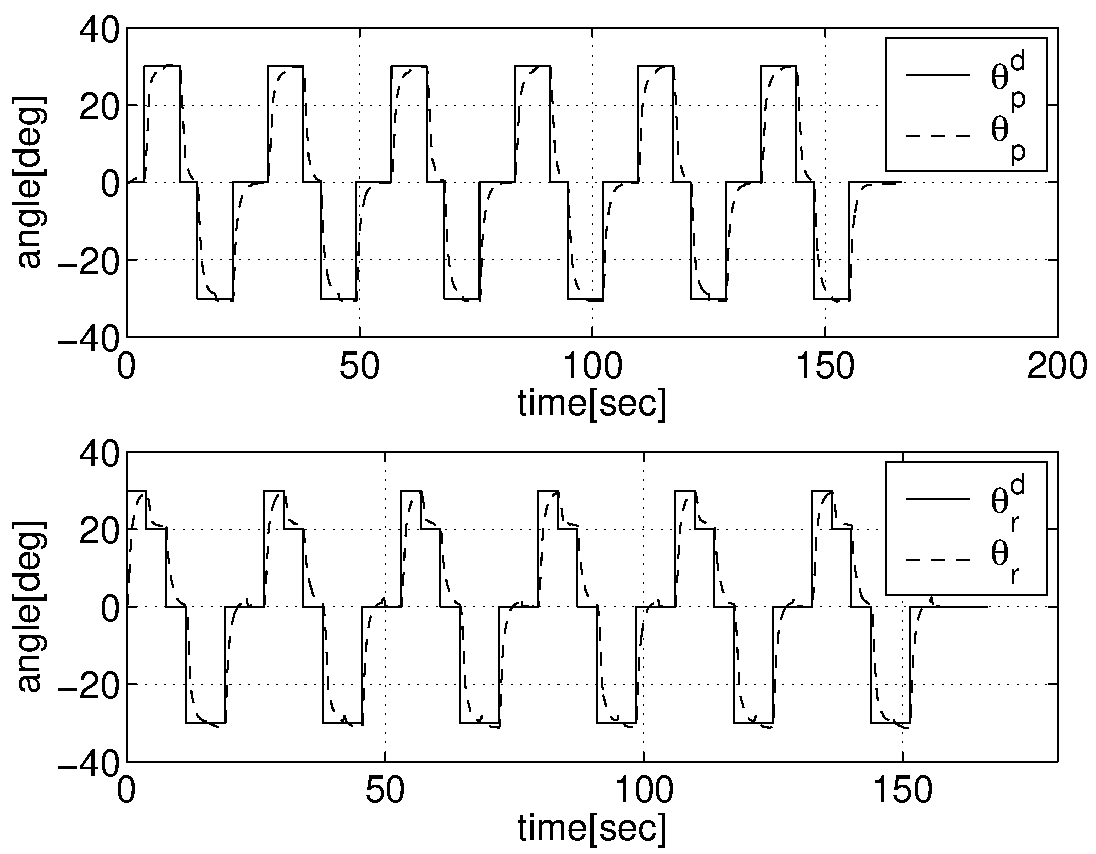
\includegraphics[width=60mm]{image/AngleModel.pdf} 
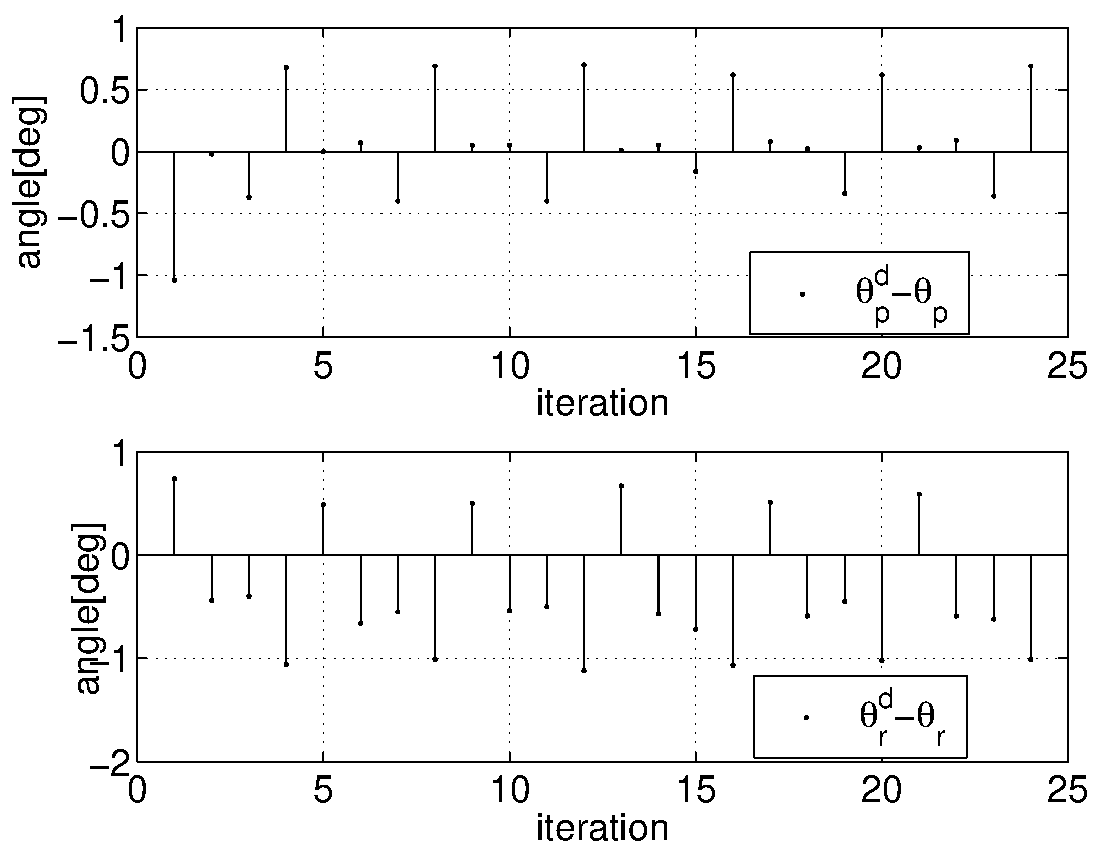
\includegraphics[width=60mm]{image/ErrorsModel.pdf} 
\caption{Evaluation of the model. The right pictures show the errors $\mathbf e = \x - \x_d = [\theta_p - \theta_p^d, \theta_r - \theta_r^d]$ in performing a sequence of movements $\x_d = [30, 0] \rightarrow[20, 30] \rightarrow[0, 30] \rightarrow[-30, 0] \rightarrow[-30, -30] \rightarrow[0, -30]$. The sequence is repeated four times as shown in the left picture. The observed root mean squared error (RMSE) is $0.43deg$ for the pitch and $0.72deg$ for the roll.}
\label{Fig:ErrorModel}
\end{figure}

\subsubsection{Jacobian based solution} \label{Sec:JacobianSolution}

In order to improve the positioning errors shown in Figure \ref{Fig:ErrorModel} we need to use the sensor measurement $\x$ as a feedback signal to reach the desired pose $\x_d$. A typical control structure for guaranteeing $\x \rightarrow \x_d$ is the following (see \cite{SamsonEspiau} for details):
\begin{equation} \label{Eq:JacobianControl}
\dot{\q} = - J_R(\q) (\x - \x_d),
\end{equation}
where $J \in \mathbb R^{2 \times 3}$ is the jacobian of (\ref{Eq:Fwd_model_neck}), and $A_R \in \mathbb R^{n \times m}$ denotes a right inverse of a matrix $A \in \mathbb R^{m \times n}$, i.e. $A A_R = I$. In our case, we do not have direct access to $J$ since we do not have an analytical expression for the function $f$ in (\ref{Eq:Fwd_model_neck}). All we have is $f_{inv}$ whose jacobian $J_{inv}$ is somehow related to $J$. Specifically, it can be shown that:
\begin{equation} \label{Eq:JacobianInv}
J(f_{inv}(\x)) J_{inv} (\x) = I \qquad \forall \x \in \mathbb R^2,
\end{equation}
which implies that $J_{inv}$ is a right inverse for  $J$ in every $\q$ belonging to the manifold $\mathcal M$ described by (\ref{Eq:Model_neck}). Therefore, if we remain on that manifold, we can use $J_{inv}$ in place of $J_R$ in Eq. (\ref{Eq:JacobianControl}). The final control law will be the following:
\begin{equation} \label{Eq:JacobianControlFinal}
\dot{\q} = - J_{inv}(\x) (\x - \x_d).
\end{equation}
Remarkably, the time derivative $\dot{\q}$ belongs to the tangent plane of $\mathcal M$ in $\mathbf q$. As a consequence of this fact, if the $\q(0) \in \mathcal M$ then $\q(t) \in \mathcal M$, $\forall t > 0$. Therefore, (\ref{Eq:JacobianControlFinal}) is exactly equivalent to (\ref{Eq:JacobianControl}) and convergence of $\x$ to $\x_d$ is guaranteed. However, from a practical point of view, the implementation of (\ref{Eq:JacobianControlFinal}) is obtained with a digital controller so that the commanded velocity $\dot{\q}$ is not continuously modified but only updated every $T_s = 0.01$ seconds, the controller rate. Therefore, we are not guaranteed that the system configuration remains on $\mathcal{M}$. Figure \ref{Fig:ErrorJacobian} shows the performance of the discrete time controller. Positioning errors are greatly improved with respect to the previously proposed controller (\ref{Eq:PurelyModelBasedControl}); the pitch RMSE has been reduced from $0.43deg$ to $0.09deg$ while the roll RMSE from $0.72deg$ to $0.05deg$. However, as a consequence of the discretization of the controller, the system is not guaranteed to remain on $\mathcal M$ as shown in Figure \ref{Fig:ManifoldDistanceJacobian}. 

\begin{figure}[tbp]
\centering 
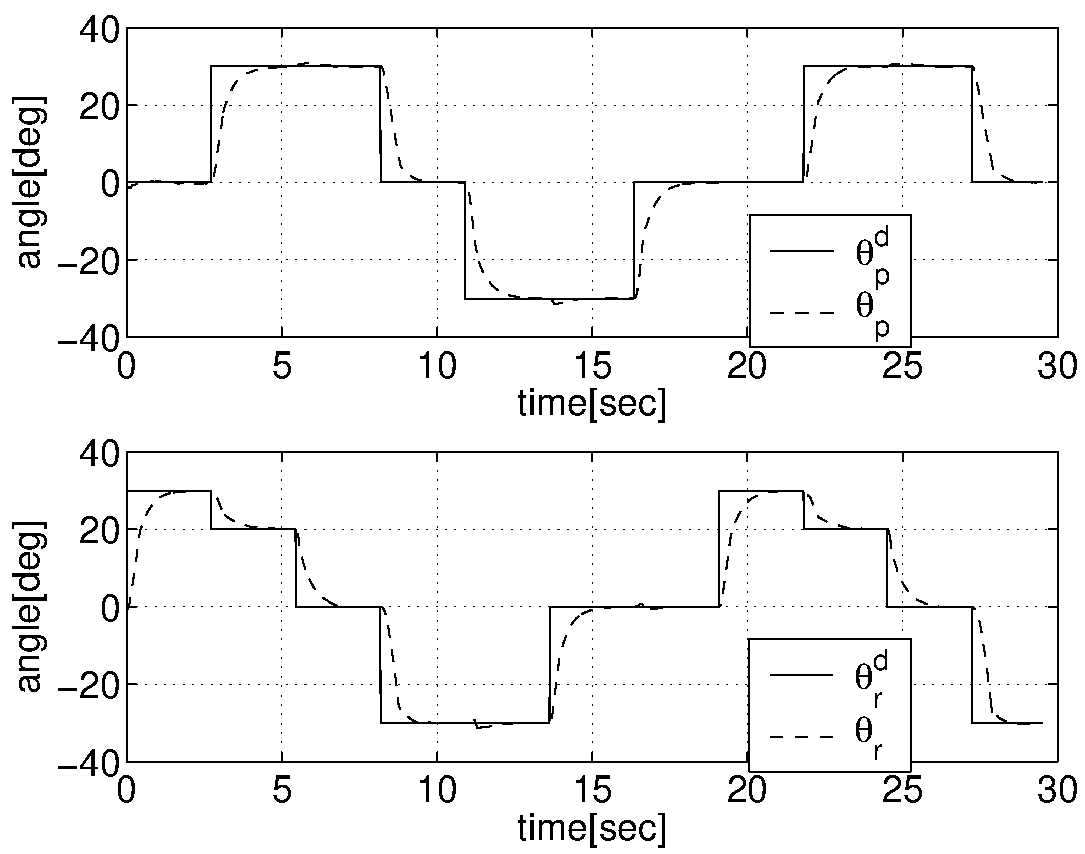
\includegraphics[width=60mm]{image/AngleJacobian.pdf} 
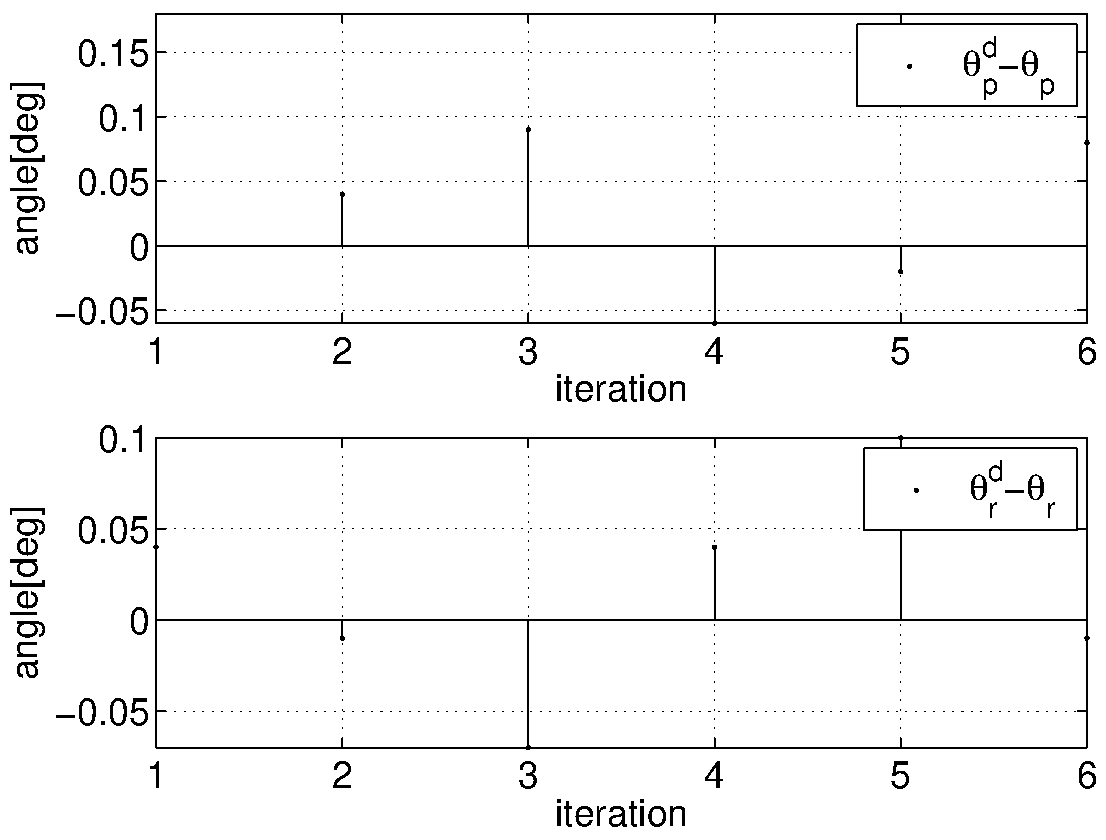
\includegraphics[width=60mm]{image/ErrorsJacobian.pdf} 
\caption{Evaluation of the closed loop controller. The right pictures show the errors $\mathbf e = \x - \x_d = [\theta_p - \theta_p^d, \theta_r - \theta_r^d]$ in performing a sequence of movements $\x_d = [30, 0] \rightarrow[20, 30] \rightarrow[0, 30] \rightarrow[-30, 0] \rightarrow[-30, -30] \rightarrow[0, -30]$. The actual movement is shown in the left pictures. The observed root mean squared error (RMSE) is $0.09deg$ for the pitch and $0.05deg$ for the roll.}
\label{Fig:ErrorJacobian}
\end{figure}

\begin{figure}[tbp]
\centering 
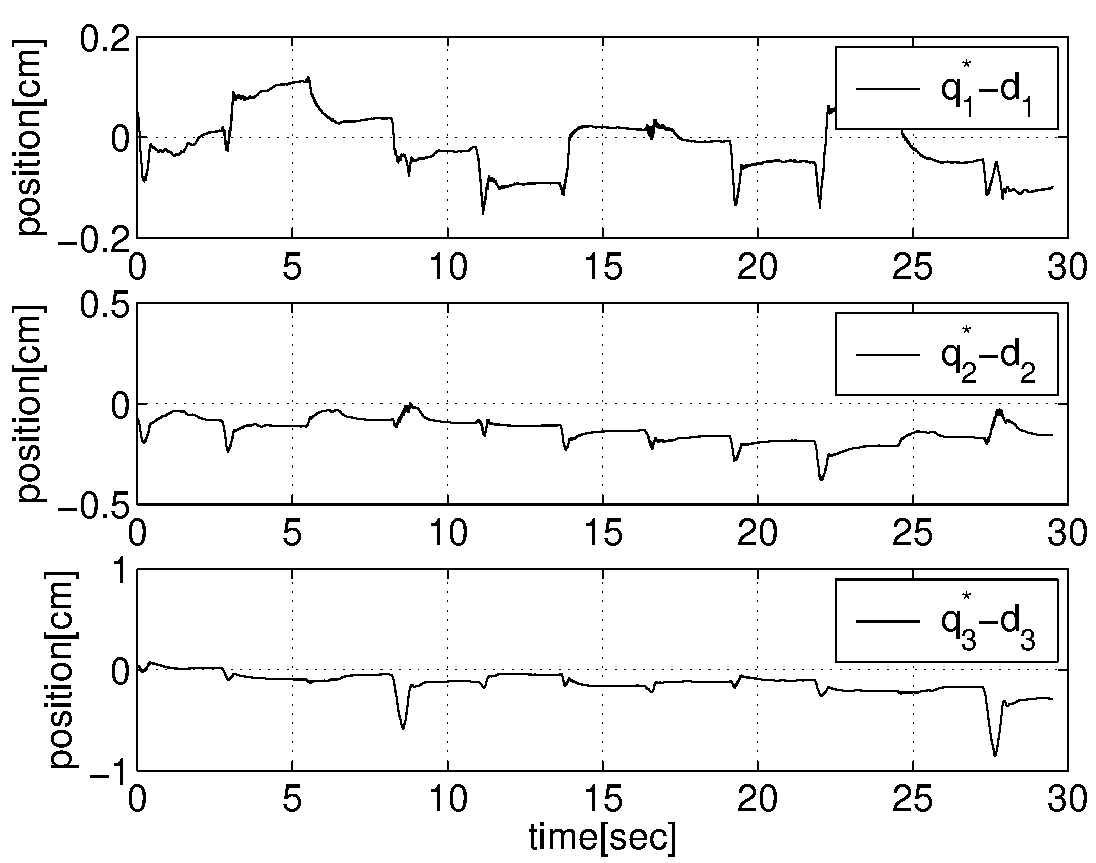
\includegraphics[width=60mm]{image/ManifoldDistanceQJacobian.pdf} 
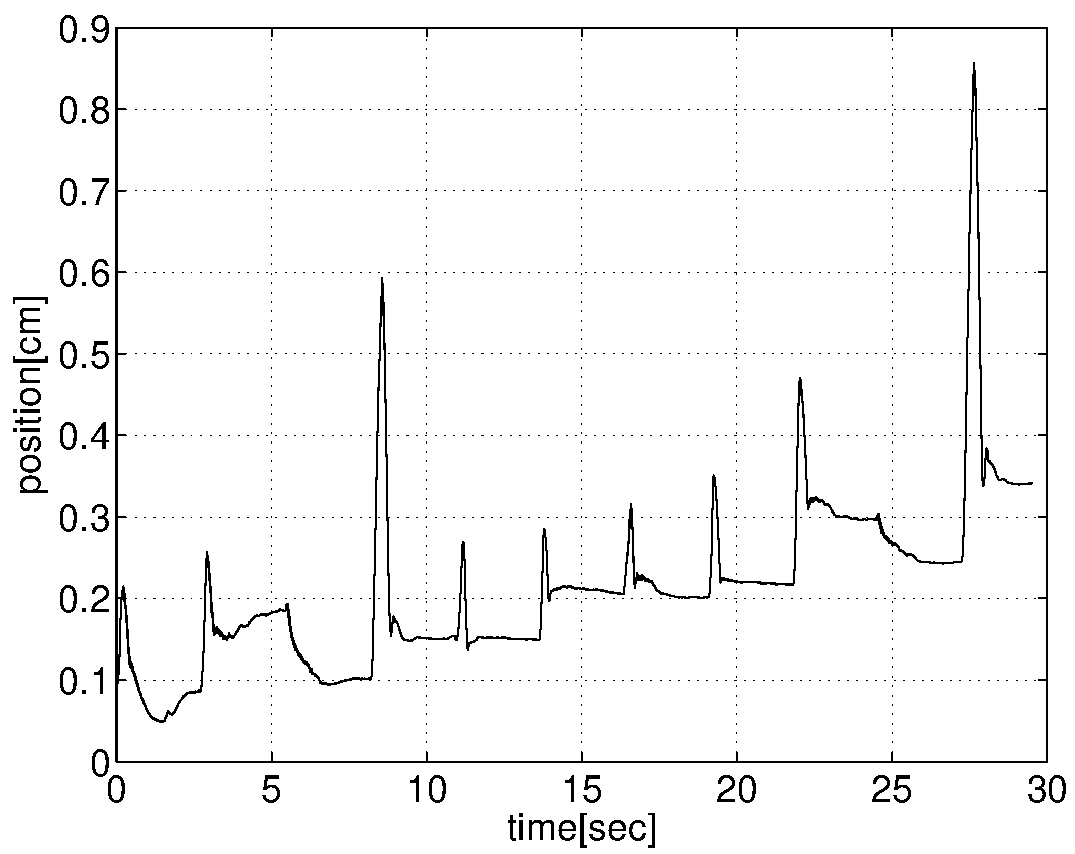
\includegraphics[width=60mm]{image/ManifoldDistanceJacobian.pdf} 
\caption{Distance of $\q$ from the manifold $\mathcal M$. The left picture shows the three components of the vector $f_{inv}(\x) -\q  = \q^* -\q$ during the movement described in Figure \ref{Fig:ErrorJacobian}. The right picture shows instead the time behaviour of its norm , i.e. $\| \q^* - \q \|$. As expected the system configuration progressively abandons the manifold.}
\label{Fig:ManifoldDistanceJacobian}
\end{figure}

\subsubsection{Weighted solution} \label{Sec:WeightedSolution}

Keeping the system configuration on the manifold $\mathcal M$ is important for the reasons illustrated in Section \ref{Sec:NeckControlInDetails}. Therefore the solution proposed in the previous section is not desiderable. According to Figure 
\ref{Fig:ManifoldDistanceJacobian} the longer we control the system the bigger becomes the distance from manifold, and from a practical point of view, the spring neck might be bent in wrong configuration or the tendons might loose their correct alignment with the capstans. The first solution to this problem is a mixture of the two proposed controllers (\ref{Eq:PurelyModelBasedControl}) and (\ref{Eq:JacobianControlFinal}):
\begin{equation} \label{Eq:WightedControl}
\dot{\q} = -\mu K_p(\q - f_{inv}(\x_d)) - (1-\mu) J_{inv}(\x) (\x - \x_d),
\end{equation}
where $\mu \in [0, 1]$ is an arbitrary weighting scalar factor and the other quantities have been defined in the previous sections. Choosing the value of the variable $\mu$ is not an easy task since it is meant to privilege either the distance to the manifold ($\mu \simeq 1$) or the achievement of a precise positioning ($\mu \simeq 0$). Choosing $\mu \simeq 0.5$ leads to the results in Figure \ref{Fig:ManifoldDistanceJacobianAndCompromise}. Remarkably the distance from the manifold is reduced (the observed RMSE is $0.1cm$) at the cost of an increased error in the positioning: the pitch-RMSE drops down from $0.09deg$ to $1.32deg$, while the roll-RMSE from $0.05deg$ to $1.17deg$.

\begin{figure}[tbp]
\centering 
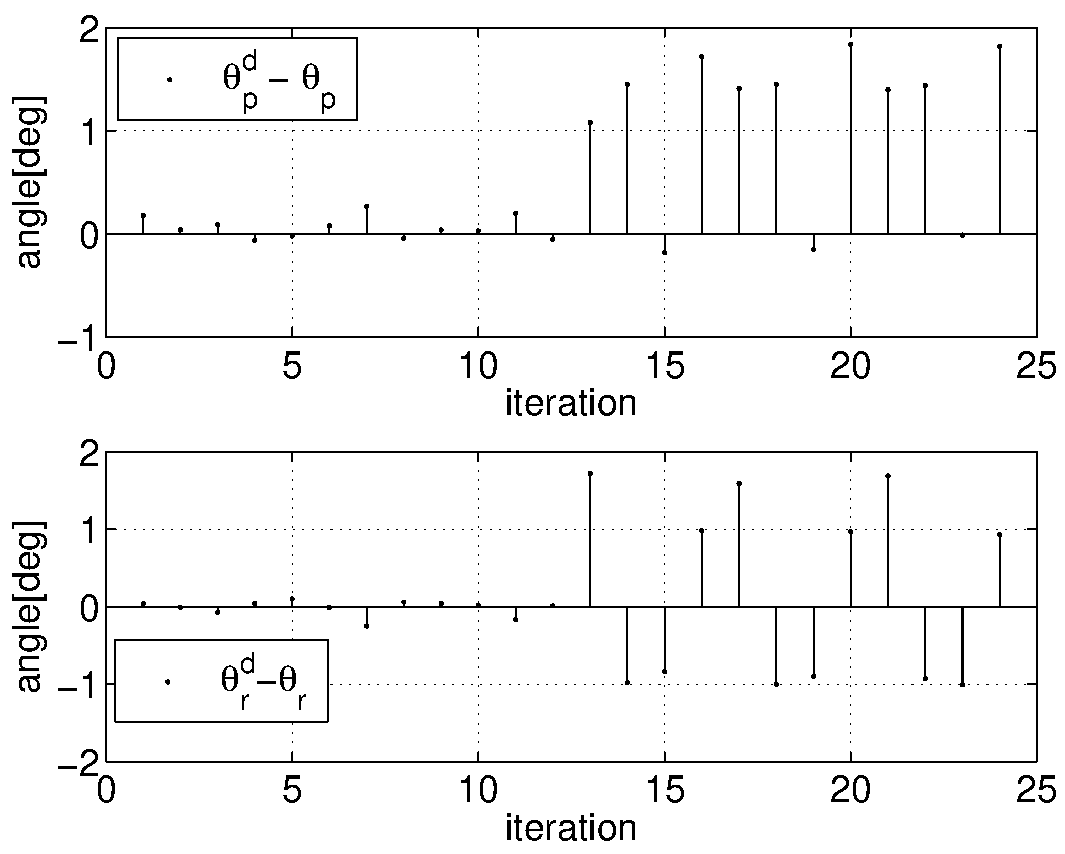
\includegraphics[width=60mm]{image/ErrorsJacobianAndComprormise.pdf} 
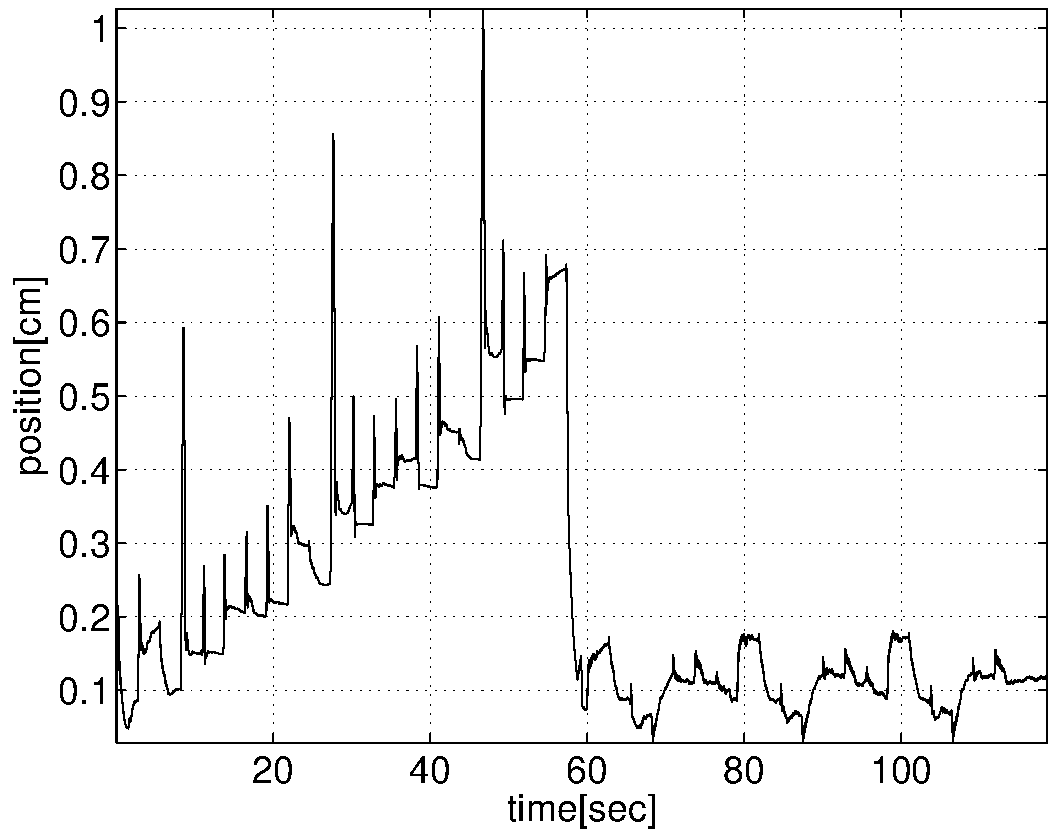
\includegraphics[width=60mm]{image/ManifoldDistanceJacobianAndComprormise.pdf} 
\caption{Right image: positioning errors $\x - \x_d$ for the two components of $\x = [\theta_p, \theta_r]$; left image: distance of $\q$ from the manifold $\mathcal M$. The usual sequence of movements has been repeated twice with the controller (\ref{Eq:JacobianControl}) and twice with \eqref{Eq:WightedControl}. The switching between the two controllers happens after about 60 seconds causing a rapid fall of the distance from the manifold.} 
\label{Fig:ManifoldDistanceJacobianAndCompromise}
\end{figure}

\subsubsection{Minimization solution} \label{Sec:MinimizationSolution}

The control law (\ref{Eq:WightedControl}) is always a compromise between accuracy in positioning and accuracy in remaining close to the manifold $\mathcal M$. Practically, we cannot achieve both tasks simultaneously because the definition of $\mathcal M$ is based on a model of the system which is usually affected by modeling errors. The best way to satisfy both tasks simultaneously consists in requiring accurate positioning ($\x=\x_d$) while requiring the system configuration $\q$ to be as close as possible to the manifold configuration $\q^* = f_{inv}(\x)$. Practically, to reach the orientation $\x_d$ we should move the system to the configuration:
\begin{equation} \label{Eq:MinimizationControlTheory}
\q_d = \min_{\q} \frac{1}{2}\| \q - f_{inv}(\x_d)\|^2, \qquad f(\q) = \x_d.
\end{equation}
The so called resolved motion rate control technique (see \cite{SamsonEspiau} for details and proof of convergence) can be used to solve the above problem:
\begin{equation} \label{Eq:MinimizationControl}
\dot{\q} = -J_R(\q) (\x-\x_d) - \left(I-J_R(\q) J_R^\dagger(\q)\right) \left(\q - f_{inv}(\x_d)\right),
\end{equation}
where $J_R$ is a right inverse of the Jacobian $J = \frac{\partial f}{\partial \q}$ and $J_R^\dagger$ is its Moore-Penrose pseudo-inverse. This control strategy can be proved to guarantee that $\q$ converges to the solution $\q_d$ of (\ref{Eq:MinimizationControlTheory}). Once more, an implementation of \eqref{Eq:MinimizationControl} on our system is complicated by the fact that we have access neither to the function $f$ nor to its Gacobian $J$. Using the same idea proposed before we have that as long as we stay on the manifold the following relationship holds: $J_R = J_{inv}$. Therefore, we can implement \eqref{Eq:MinimizationControl} as follows:
\begin{equation} \label{Eq:MinimizationControl2}
\dot{\q} = -J_{inv}(\x) (\x-\x_d) - \left(I-J_{inv}(\x) J_{inv}^\dagger(\x)\right) \left(\q - f_{inv}(\x_d)\right).
\end{equation}
Clearly, \eqref{Eq:MinimizationControl2} is similar to \eqref{Eq:WightedControl} but in this case the manifold distance is controlled by performing movements in the null space of the primary task, the neck orientation. Theoretically, \eqref{Eq:MinimizationControl} will be equal to \eqref{Eq:MinimizationControl2} only if we guarantee to remain on the manifold. Practically, all we are interested in is the convergence of the control to the desired final configuration; farily weack conditions to guarantee the convergence can be found in \cite{SamsonEspiau}. These conditions\footnote{In practice convergence is guaranteed if $J J_{inv} >0$ which is obviously true on the manifold $\mathcal M$ where $J_{inv} = J_R$ so that we have $J J_{inv} = I$.} can be used to prove convergence of the proposed control scheme under the assumption that the system configuration remains close enough to $\mathcal M$. Further and more formal investigations on this sketch of convergence proof will be given on a forthcoming paper.



\section{Future work} \label{Sec:FutureWork}

Preliminary works have been carried out concerning the development of a non-model-based controller for James neck.\\The planned solution makes use of a Receptive Fields Neural Network to estimate the joint-space velocities needed to move the head with the desired task-space velocities, given the actual joint configuration. The learning algorithm is an implementation, with some modifications, of the Receptive Fields Weighted Regression proposed by Schaal and Atkenson \cite{Schaal98rfwr}.\\After a training phase, in which the workspace is randomly explored by the robot and the network learns on-line from the gathered sensory data, the trained network is able to map the two spaces. This mapping is called, in mathematical terms, the global inverse Jacobian matrix.\\Unfortunately, due to the redundant actuation system we deal with, our Jacobian matrix is not square, and so not invertible. This means that for a given set of actual joints positions and required task-space velocities there is not a unique solution in terms of joint-space velocities; nevertheless, within this family of solutions, just a very limited set is usable in practice, because a minimum amount of tension is needed along the tendons to avoid their possible outgo from the capstans.\\To overcome this problem, the velocities applied to the motors during the training phase result from the summation of two weighted terms: the first is a random one, and has a bigger weight, and the second tries to keep a suitable tension along the tendons, acting in the null-space of the Jacobian.\\A first stage of development for the discussed controller has been already reached, and an initial version has been tested on James. Results show that the system is able to learn a good approximation of the inverse Jacobian after a training stage of about a hour. The trained controller allows the head to reach the desired equilibrium position in the task-space, with logarithmic velocity profiles and a satisfying degree of accuracy.


\section{Conclusions} \label{Sec:Conclusions}
We proposed an innovative neck mechanical structure which is highly biologically inspired. The main idea is to have a flexible structure (neck bone) actuated by surrounding compressive elements (muscles). In the specific implementation the flexible structure is represented by a steel spring. Its actuation is achieved with standard dc motors which are used to pull three tendons surrounding the neck. The final structure is capable of bending the neck roughly around a sphere. This new mechanical design has required the development of an appropriate control structure which uses an orientation tracker, a model of the system kinematics and a Jacobian based feedback loop. The peculiarity of the system made it difficult to model directly its forward kinematics; practically, it was easier to model a specific solution of the inverse kinematics. On the basis of this solution, a suitable control strategy was proposed and implemented on the real robot. A formal mathematical proof of the convergence of the proposed control scheme was not given even if simple considerations seem to pave the way to a complete formal proof. In any case the controller has been practically shown to work in line with the required performance.

\appendix 

\section{Partial inverse kinematics modeling}
The three main assumptions are the following: the spring length is constant (remember that the spring is completely compressed by the head weight), it assumes a constant curvature and it always lays (??????????) on a plane. Only the two extremities of the spring are attached to the robot, one to the fixed base of the neck (reference frame $\Sigma_b$) and the other to a movable plane on which the orientation tracker (reference frame $\Sigma_s$) is mounted (see also Figure \ref{Fig:HeadAct}). Practically the sensor measures the orientation of the this plane with respect to the gravitational force vector. In the remaining of this section, we express the sensor measurement in terms of the $\mathbf z$-axis of the reference frame $\Sigma_s$. Given the configuration of the system, this axis, denoted $\mathbf z_s$, is always parallel to gravity and can be easily expressed in terms of $\theta_p$ and $\theta_r$:
$$ \mathbf z_s = \begin{bmatrix}  -\sin(\theta_r) & \sin(\theta_p)\cos(\theta_r) & -\cos(\theta_p)\cos(\theta_r)\end{bmatrix}^\top.$$
In order to compute the function $f_{inv}$ which expresses the tendons length $\q$ given the sensor measurement $\x$, we proceed by computing the position of $\Sigma_s$ as a function of $\x$. Remarkably, notice that the orientation of $\Sigma_s$ is already known given that $\mathbf z_s$ is known and the system does not rotate with respect $\mathbf z_s$. Therefore we are left with determining the translation of $\Sigma_s$, or equivalently the position of its origin $O_s$ with respect to $\Sigma_b$. The first problem to solve consists in finding the plane $\mathcal P$ on which the spring lays (??????). Given  the assumptions, $\mathcal P$ is orthogonal to $\mathbf z_b$ and $\mathbf z_s$ and passes trough the origin $O_b$ of $\Sigma_b$. These considerations easily follow from the fact that the spring extremities are always orthogonal to the planes on which they are attached. Therefore, $\mathcal P$ is uniquely determined by its normal $\mathbf z_n = \mathbf z_s \times \mathbf z_b$ and one of its points $O_b$. Once $\mathcal P$ has been uniquely determined we only need to determine the position of $O_s$ within this plane. This is a two dimensional problem and can be easily illustrated (Figure \ref{Fig:HeadActCalc}). We now restrict to the 2D case since the extension to 3D is just a matter of a rotation. Practically speaking, the spring describes an arc of a circle (see Figure \ref{Fig:HeadActCalc}) whose length is $L$ (the length of the compressed spring) and whose angular amplitude is $\theta = \mbox{arcos}(\mathbf z_b \cdot \mathbf z_b) $. The radius of this circle is therefore:
$$ R = \frac{L}{\theta}.$$
Considering a two dimensional reference frame $(\mathbf y_{\mathcal P}, \mathbf z_{\mathcal P})$ with origin in $O_b$, the relative position between $O_b$ and $O_s$ is described by the vector $[(R+R_s) (1 - \cos(\theta), (R+R_s) \sin(\theta)]$ being $R_s$ the spring radius. This vector can be used to describe the position of $O_s$ with respect to $\Sigma_b$ and therefore the relative position between $\Sigma_b$ and $\Sigma_s$. Once this position is known we can compute the cables length $\q$ given the system kinematic parameters; in particular we have $\q = \begin{bmatrix} |E_1-P_1|, & |E_2-P_2|, & |E_3-P_3| \end{bmatrix} $ (see Figure \ref{Fig:HeadActCalc}) where $E_i$ are all fixed in $\Sigma_s$ and $P_i$ are all fixed in $\Sigma_b$.


\begin{figure}[tbp]
\centering
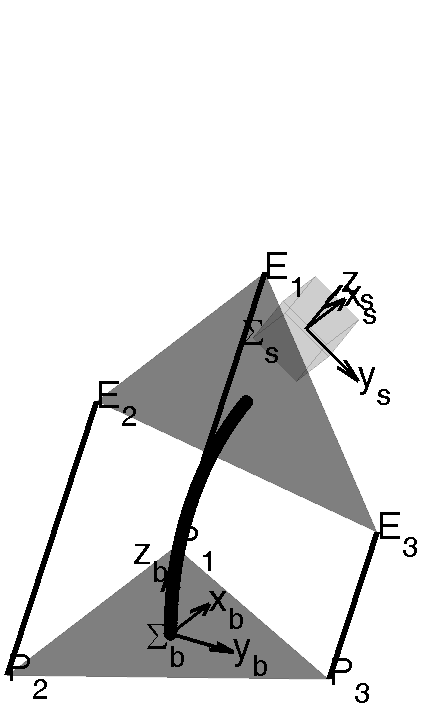
\includegraphics[width=30mm]{image/NeckModel.pdf} 
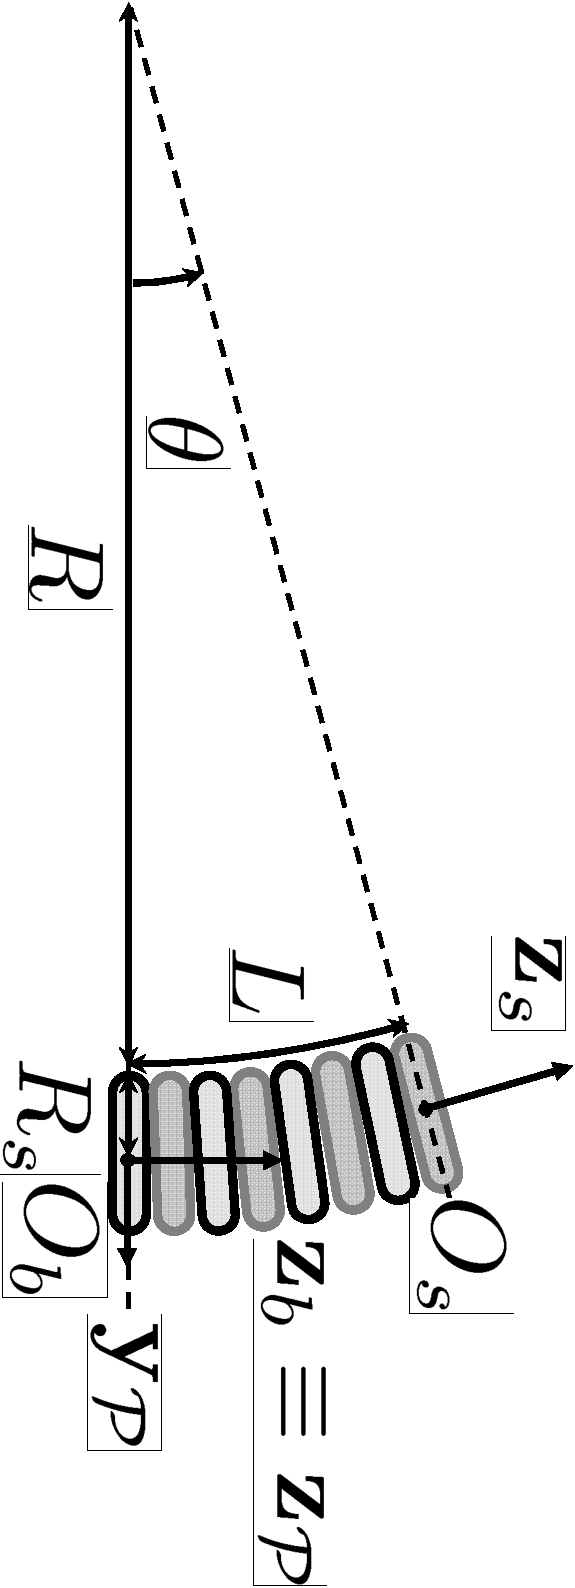
\includegraphics[width=20mm, angle=90]{image/NeckModelCalc.pdf} 
\caption{Scheme for computing the inverse kinematic function $f_{inv}$. On the right picture, everything has been reduced to plane $\mathcal P$ to which both $\mathbf z_s$ and $\mathbf z_b$ belong.}
\label{Fig:HeadActCalc}
\end{figure}


\bibliographystyle{plain}
\bibliography{MyBiblio}
\end{document}